\chapter{Struttura di openHAB}
\begin{figure}
    \centering
    
\includegraphics{Immagini/openhab_logo.png}
    \caption{openHAB Logo}
    \label{fig:openhab_logo}
\end{figure}

Per cominciare ad utilizzare {\em openHAB } bisogna eseguire dei passaggi iniziali
\begin{enumerate}
    \item possedere un \textbf{computer} sul quale eseguire il software. Vi sono molti device disponibili per eseguire openHAB. Il più minimale e famoso è sicuramente \textbf{Raspberry Pi} perché integra perfettamente \textbf{openHABian}, ovvero una distribuzione {\em Linux} completamente auto-configurata per soddisfare le esigenze degli utenti openHAB. Essa contiene l'immagine completa della scheda SD già preconfigurata e lo strumento di configurazione openHABian. Un altro dispositivo molto diffuso sul quale eseguire {\em openHAB} è \textbf{DiskStation di Synology}, ovvero un server NAS. Tale approccio è meno economico ma migliore se già si possiede tale dispositivo. OpenHAB può essere eseguito anche su un normale \textbf{computer domestico} anche se è preferibile utilizzare un sistema dedicato.
    \item installare {\em openHAB} e i vari \textbf{software} per farlo funzionare. {\em OpenHAB} è stato scritto in {\em java}, dunque dipende dalla {\em Java Virtual Machine}. La JVM è disponibile di default nei nuovi dispositivi, in caso contrario bisogna scaricarla. La versione attualmente supportata è la \textbf{JVM Java 11} e \textbf{Azul Zulu} è la piattaforma consigliata per {\em openHAB}. Il software openHAB è disponibile per diverse versioni \textbf{macOS} e \textbf{Windows} e molte distribuzioni \textbf{Linux} come {\em Ubuntu}, {\em Raspbian}, ... Dopo aver installato il software vi sono passi aggiuntivi da fare come configurare una rete condivisa per editare in maniera agevole i file di configurazione. Per tale scopo viene utilizzato {\em Linux Samba Share} lato server, mentre lato client {\em Visual Studio Code} con {\em openHAB VS Code Extension}.
    \item far interagire i vari \textbf{dispositivi smart} con il server {\em openHAB}. Un dispositivo intelligente è un dispositivo elettronico, generalmente connesso ad altri dispositivi o reti tramite diversi protocolli. {\em OpenHAB} permette di collegarsi direttamente a loro e gestirli in maniera semplice e automatizzata.
\end{enumerate}

\section{Concetti Principali}
\begin{table}[]
    \centering
    \begin{tabular}{ l | p{10cm} }
        \textbf{Concetto} & \textbf{Descrizione}\\
        \hline
         Binding &  sono i componenti openHAB che forniscono l'interfaccia per interagire elettronicamente con i dispositivi\\
         Things & sono la prima rappresentazione generata da openHAB dei dispositivi\\
         Channels & sono la connessione openHAB tra ``Things'' e ``Items''\\
         Items & sono la rappresentazione generata da openHAB delle informazioni sui dispositivi\\
         Rules & vengono eseguite azioni automatiche (nella forma più semplice: se ``questo'' accade, openHAB farà ``quello'')\\
         Sitemap & interfaccia utente (sito web) generata da openHAB che presenta le informazioni e consente le interazioni
    \end{tabular}
    \caption{Concetti}
    \label{tab:concetti}
\end{table}

I concetti principali sono rappresentati nella Tabella \ref{tab:concetti}.

\subsection{Binding} \label{chap:binding_intro} Sono pacchetti software installati dall'utente che hanno lo scopo di stabilire una connessione tra il dispositivo e la thing. Essi traducono tutti i comandi tra {\em openHAB} e la {\em thing}. I binding sono elencati nella sezione {\em Add-on} della documentazione ufficiale. Per ogni {\em binding} vengono fornite istruzioni dettagliate ed esempi che includono una guida alla configurazione dell'associazione, l'elenco delle {\em things} supportate e i {\em channels} che le {\em things} forniscono.

\subsection{Things} Sono le entità che possono essere fisicamente connesse al sistema e che potenzialmente forniscono più di una funzionalità. Esse non sono identificabili come device ma come il web service che questi che queste possiedono per essere controllate. Le {\em things} sono rilevanti per i processi di setup e configurazione ma non a runtime. Esse possono avere sia proprietà facoltative che obbligatorie (come indirizzo ip, access token, ...).

Un tipo particolare di {\em thing} è un \textbf{bridge}. Essi sono {\em thing} che devono essere aggiunte al sistema per aver accesso ad altre {\em thing}. 

Poiché molte {\em things} possono essere scoperte automaticamente, sono disponibili meccanismi speciali che si occupano di tale gestione.

Ogni {\em thing} ha uno stato che aiuta a identificare possibili problemi con il dispositivo o il servizio. Possiamo vedere l'elenco degli stati alla Tabella \ref{tab:things_states}.

\begin{table}[]
    \centering
    \begin{tabular}{ l | p{10cm} }
        \textbf{State} & \textbf{Descrizione}\\
        \hline
        UNINITIALIZED & Stato iniziale di una {\em thing} quando viene aggiunta o il framework viene avviato. Questo stato viene assegnato anche se il processo di inizializzazione non è riuscito o l'associazione non è disponibile. I comandi inviati ai {\em channels} non verranno elaborati.\\
        INITIALIZING & Stato che viene assegnato mentre l'associazione inizializza la  {\em thing}. Dipende dall'associazione quanto tempo impiega il processo di inizializzazione. I comandi inviati ai {\em channels} non verranno elaborati.\\
        UNKNOWN & Il device è completamente inizializzato ma, a causa della natura del dispositivo/servizio rappresentato, non è ancora in grado di dire realmente se la thing è ONLINE o OFFLINE. Pertanto, la {\em thing} potrebbe già funzionare correttamente e potrebbe o non potrebbe elaborare i comandi. Ma il framework è autorizzato a inviare comandi, perché alcuni dispositivi basati su radio possono andare ONLINE se viene inviato loro un comando. Il conduttore dovrebbe aver cura di passare la {\em thing} a ONLINE o OFFLINE il prima possibile.\\
        ONLINE & Si presume che il dispositivo/servizio rappresentato da una {\em thing} funzioni correttamente e possa elaborare i comandi.\\
        OFFLINE & Si presume che il dispositivo/servizio rappresentato da una {\em thing} non funzioni correttamente e potrebbe non elaborare i comandi. Ma il framework è autorizzato a inviare comandi, perché alcuni dispositivi basati su radio potrebbero tornare a ONLINE se viene inviato loro un comando.\\
        REMOVING & Il dispositivo/servizio rappresentato da una {\em thing} dovrebbe essere rimosso, ma l'associazione non ha ancora confermato l'eliminazione. Alcune associazioni devono comunicare con il dispositivo per annullarne l'associazione dal sistema. Probabilmente la {\em thing} non funziona e i comandi non possono essere elaborati.\\
        REMOVED & Stato indicante che il dispositivo/servizio rappresentato da una {\em thing} è stato rimosso dal sistema esterno dopo che la REMOVING è stata avviata dal framework. Di solito tale stato è uno stato intermedio perché la {\em thing} viene rimossa dal database dopo che esso è stato assegnato.
    \end{tabular}
    \caption{Things states}
    \label{tab:things_states}
\end{table}

\begin{figure}
    \centering
    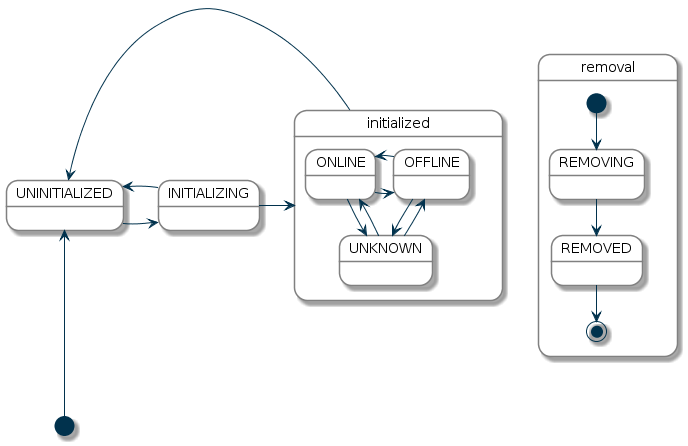
\includegraphics[width=12cm]{Immagini/status_transitions}
    \caption{Transizioni di Stato}
    \label{fig:status_transitions}
\end{figure}

Gli stati UNINITIALIZED, INITIALIZED, REMOVING e REMOVED sono impostati dal framework mentre UNKNOWN, ONLINE e OFFLINE sono assegnati dal binding. Sono rappresentate le transizioni tra i vari stati alla Figura \ref{fig:status_transitions}.

\subsection{Channels} Vengono forniti dalle {\em things} e rappresentano le diverse loro funzioni. Dove la {\em thing} è un'entità fisica o la fonte di informazione, il {\em channel} è una funzione concreta di questa. Una lampadina fisica({\em thing}) potrebbe avere un canale della temperatura del colore({\em channel 1}) e un canale del colore({channel 2}), che forniscono entrambi la funzionalità dell'unica {\em thing} della lampadina al sistema. Per le fonti di informazione, la {\em thing} potrebbe essere il tempo locale con informazioni da un servizio web con diversi {\em channels} come temperatura, pressione e umidità. I {\em channels} sono collegati agli {\em items} e questi collegamenti sono il collante tra livello fisico e virtuale. Stabilito il collegamento una {\em thing} reagisce agli eventi inviati per un {\em item} collegato ad uno dei suoi {\em channels} e a sua volta una {\em thing} può inviare eventi attraverso gli {\em item} sfruttando uno dei suoi {\em channel}.

\subsection{Items} {\em OpenHAB} applica una forte separazione tra mondo fisico ({\em Things}) e mondo virtuale ({\em Items}). Gli {\em Items} rappresentano in particolarità le funzionalità usate dall'applicazione. Essi hanno uno {\em stato} e vengono usati attraverso degli {\em eventi}. Gli {\em Items} disponibili sono rappresentati alla Tabella \ref{tab:items}.

\begin{table}[]
    \centering
    \begin{tabular}{l|p{5cm}|p{5cm}}
        \textbf{Nome Item} & \textbf{Descrizione} & \textbf{Tipo di Comando} \\
        \hline
        Color & Informazione sul colore(RGB) & OnOff, IncreaseDecrease, Percent, HSB\\
        Contact & Stato di memorizzazione dell'articolo & OpenClosed\\
        DateTime & Memorizzazione data e ora & -\\
        Dimmer & Valore percentuale del dimmer & OnOff, IncreaseDecrease, Percent\\
        Group & Oggetto che ne raccoglie altri & -\\
        Image & Contiene i dati binari dell'immagine & -\\
        Location & Memorizza le coordinate GPS & Point\\
        Number & Memorizza valori nel formato numero e può avere una dimensione opzionale per il suffizzo & Decimal\\
        Number:\textless dimension\textgreater & Come Number ma con un'informazione addizionale per l'unità supportata & Quantity\\
        Player & Permette di controllare i players come i riproduttori musicali & PlayPause, NextPrevious, RewindFastforward\\
        Rollershutter & Tipicamente utilizzati per le tapparelle & UpDown, StopMove, Percent\\
        String & Memorizza testi & String\\
        Switch & Usati tipicamente per le luci & OnOff
    \end{tabular}
    \caption{Items}
    \label{tab:items}
\end{table}

Gli {\em items} \textbf{group} possono contenere {\em items} o {\em groups} al loro interno. In questo modo a livello di interfaccia utente viene vista una sola voce per il {\em group} che poi può fornire in dettaglio la vista di ogni singolo membro. Il raggruppamento ciclico non è vietato ma fortemente sconsigliato. Un esempio rappresentante la configurazione di un gruppo è alla Figura \ref{fig:group_item_example}.

\begin{figure}
    \centering
    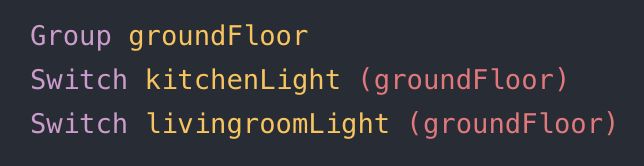
\includegraphics{Immagini/GroupItemExample}
    \caption{Esempio Group Item}
    \label{fig:group_item_example}
\end{figure}

{\em Group items} possono derivare il proprio stato dai loro membri; per fare ciò i {\em group} devono essere costruiti a partire da un {\em base item} e una {\em group function}. Nel calcolare lo stato la {\em group function} attraversa i membri di gruppi e sottogruppi e se trova un {\em item} che definisce lui stesso uno stato allora viene preso questo come stato del gruppo.

Il {\em formato} dei vari {\em items sarà}
\begin{itemize}
    \item \textbf{StringType}: normali java strings
    \item \textbf{DateTimeType}: java SimpleDateFormat.parse() usando come matching pattern yyyy-MM-dd'T'HH:mm:ss.SSSZ, yyyy-MM-dd'T'HH:mm:ss.SSSz, yyyy-MM-dd'T'HH:mm:ss.SSSX, yyyy-MM-dd'T'HH:mm:ssz, yyyy-MM-dd'T'HH:mm:ss
    \item \textbf{DecimalType, PercentType}: java BigDecimal e java PercentType con valori tra 0 e 100
    \item \textbf{QuantityType}: valore numerico più un unità numerica
    \item \textbf{HSBType}: tre valori numerici separati dalla virgola che corrispondono a {\em Hue} (tonalità) compreso tra 0 e 360, {\em Saturation} (saturazione) compresa tra 0 e 100 e {\em Brightness} (luminosità) compresa tra 0 e 100
    \item \textbf{PointType}: sono tre valori numerici separati dalla virgola che indicano {\em latitudine}, {\em longitudine} e {\em altitudine}. I primi due vengono rappresentati in gradi mentre il terzo in metri.
    \item  \textbf{EnumTypes}: rappresentati alla Tabella \ref{tab:enum_types}
\end{itemize}

\begin{table}[]
    \centering
    \begin{tabular}{l|l}
        \textbf{Type} & \textbf{Valore supportato} \\
        \hline
        IncreaseDecreaseType & INCREASE, DECREASE\\
        NextPreviousType & NEXT, PREVIOUS\\
        OnOffType & ON, OFF\\
        OpenClosedType & OPEN, CLOSED\\
        PlayPauseType & PLAY, PAUSE\\
        RewindFastforwardType & REWIND, FASTFORWARD\\
        StopMoveType & STOP, MOVE\\
        UpDownType & UP, DOWN
    \end{tabular}
    \caption{EnumTypes}
    \label{tab:enum_types}
\end{table}

A volte è necessario allegare informazioni aggiuntive agli elementi per determinati casi d'uso. Potrebbe trattarsi di un'applicazione che necessita di alcuni suggerimenti per rendere gli {\em items} in modo generico, o un'integrazione con assistenti vocali, o qualsiasi altro servizio che accede agli {\em items} e ha bisogno di comprenderne il significato. Per questo ci sono gli {\em items metadata} che possono essere allegati agli {\em item} utilizzando namespaces. Ogni metadata è una entry che ha un valore principale o una coppia opzionale di chiave/valore (esempio: Switch MyFan "My Fan" {homekit="Fan.v2", alexa="Fan" [type="oscillating", speedSteps=3]}).

\subsection{Rules} Servono per automatizzare dei processi. Ogni regola invoca uno script che esegue dei tasks. Le {\em rules} sono nella cartella \textbf{\$OPENHAB\_CONF/rules}. Vi sono degli esempi dai quali partire nel demo file chamato {\em demo.rules}. Un file può contenere diverse regole che condividono lo stesso contesto di esecuzione. Le regole possono essere manipolate anche da UI. Ciò è possibile tramite l'accesso al web server tramite browser e andando nella sezione Settings/Rules. Quì tramite l'icona + è possibile aggiungere una nuova regola inserendo un {\em nome} e impostando un {\em trigger}. In seguito bisogna aggiungere un'azione che verrà scaturita dell'attivazione del trigger. Questa è lo script che andremo ad aggiungere. \'E possibile inserire o un ECMAScript in javascript o un Rule DSL in un linguaggio proprietario di openHAB. L'estensione {\em openHAB VS Code Extension} aiuta il programmatore a scrivere in modo corretto le {\em rules} per Rule DSL.

Il {\em rule file} è strutturato in 
\begin{itemize}
    \item Imports
    \item Variable Declarations
    \item Rules
\end{itemize}

\paragraph{Imports} sono come in java; infatti non fanno altro che importare delle librerie per usarle all'interno del file. Esempio al Codice \ref{code:rules_import}.

\begin{lstlisting}[caption=Import, label=code:rules_import]
import java.net.URI
\end{lstlisting}

\paragraph{Variable Declarations} sono variabili usate dalle {\em rules} del file. Esse possono avere o no un valore iniziale e possono essere modificabili o read-only. Esempio al Codice \ref{code:rules_variable_declarations}.

\begin{lstlisting}[caption=Variable Declarations, label=code:rules_variable_declarations]
// a variable with an initial value. Note that the variable type is automatically inferred
var counter = 0

// a read-only value, again the type is automatically inferred
val msg = "This is a message"

// an uninitialized variable where we have to provide the type (as it cannot be inferred from an initial value)
var Number x
\end{lstlisting}

\paragraph{Rules} contengono la lista di regole e la loro sintassi deve essere come quella dell'esempio al Codice \ref{code:rules_rules}

\begin{lstlisting}[caption=Rules,label=code:rules_rules]
rule "<RULE_NAME>"
when
    <TRIGGER_CONDITION> [or <TRIGGER_CONDITION2> [or ...]]
then
    <SCRIPT_BLOCK>
end
\end{lstlisting}

\begin{itemize}
    \item \textless RULE\_NAME\textgreater: ogni regola deve avere un nome univoco e possibilmente con un significato associato
    \item \textless TRIGGER\_CONDITION\textgreater: sono le condizioni tramite le quali vengono applicate le regole. Una regola viene eseguita quando si verifica la sua condizione. Possono essere aggiunte più condizioni separate dalla parola chiave {\em or}
    \item \textless SCRIPT\_BLOCK\textgreater: corrisponde alla logica che viene eseguita quando una certa condizione diventa vera
\end{itemize}

\subsubsection{Triggers}
Vi sono differenti tipi di {\em trigger} che possono essere inseriti
\begin{itemize}
    \item \textbf{Item}(-Event)-based triggers: reagiscono agli eventi sul bus degli eventi openHAB, ovvero reagiscono a comandi o aggiornamenti di stato degli {\em Items}
    \item \textbf{Member of}(-Event)-based triggers: reagiscono agli eventi sul bus degli eventi openHAB per gli {\em Items} che fanno parte del gruppo fornito
    \item \textbf{Time}-based triggers: reagiscono ad una certa ora preimpostata
    \item \textbf{System}-based triggers: reagiscono ad un certo stato del sistema
    \item \textbf{Thing}-based triggers: reagiscono ad uno stato di una {\em thing}, per esempio il cambio tra online e offline
\end{itemize}

\paragraph{Event-based Triggers}: \'E possibile ascoltare i comandi per un {\em item} specifico, sugli aggiornamenti di stato. Può essere scelto se catturare solo un comando/stato specifico o uno qualsiasi. La sintassi per questi casi è al Codice \ref{code:event-based_triggers}.

\begin{lstlisting}[caption=Event-based Triggers,label=code:event-based_triggers]
Item <item> received command [<command>]
Item <item> received update [<state>]
Item <item> changed [from <state>] [to <state>]
\end{lstlisting}

\paragraph{Member of Triggers}: come event-based triggers ma dei membri di un gruppo dato. Le variabili implicite vengono popolate dall'{\em item} che causa l'evento. La variabile {\em triggerItem} viene popolata dalll'{\em item} che ha causato il trigger della {\em rule}. Esempio al Codice \ref{code:member_of_triggers}. I {\em member of triggers} lavorano con i membri diretti di un gruppo e non con gruppi nidificati.

\begin{lstlisting}[caption=Member of Triggers,label=code:member_of_triggers]
Member of <group> received command [<command>]
Member of <group> received update [<state>]
Member of <group> changed [from <state>] [to <state>]
\end{lstlisting}

\paragraph{Time-based Triggers}: si possono usare espressioni predefinite per le ore o espressioni cronologiche. I campi di un'espressione cronologica possono essere 6 o 7:
\begin{enumerate}
    \item Seconds
    \item Minutes
    \item Hours
    \item Day-of-Month
    \item Month
    \item Day-of-week
    \item Year (opzionale)
\end{enumerate}
Un esempio è al Codice \ref{code:time-based_triggers}.

\begin{lstlisting}[caption=Time-based Triggers,label=code:time-based_triggers]
Time is midnight
Time is noon
Time cron "<cron expression>"
\end{lstlisting}

\paragraph{System-based Triggers}: si dovrebbe usare System started trigger per inizializzare i valori allo startup se non lo sono. Esempio al Codice \ref{code:system-based_triggers}.

\begin{lstlisting}[caption=System-based Triggers,label=code:system-based_triggers]
rule "Speedtest init"
when
    System started
then
    createTimer(now.plusSeconds(30), [|
        if (Speedtest_Summary.state == NULL || Speedtest_Summary.state == "") Speedtest_Summary.postUpdate("unknown")
    ])
end
\end{lstlisting}

\paragraph{Thing-based Triggers}: si possono catturare eventi di cambiamento o aggiornamento di uno stato generato da una particolare {\em thing}. Si possono catturare uno specifico aggiornamento/cambiamento di stato o qualsiasi. La sintassi è mostrata con un esempio al Codice \ref{code:thing-based_triggers}.

\begin{lstlisting}[caption=Thing-based Triggers,label=code:thing-based_triggers]
Thing <thingUID> received update [<status>]
Thing <thingUID> changed [from <status>] [to <status>]
\end{lstlisting}

\paragraph{Channel-based Triggers} alcuni add-ons forniscono dei {\em trigger channels}. Un {\em trigger channel} fornisce informazioni su eventi discreti e non continui. Si può reagire ad uno specifico o ad ogni trigger che il {\em channel} fornisce. Vi è l'esempio al Codice \ref{code:channel-based_triggers}.

\begin{lstlisting}[caption=Channel-based Triggers,label=code:channel-based_triggers]
Channel "<triggerChannel>" triggered [<triggerEvent>]
\end{lstlisting}

\subsubsection{Scripts}

Il linguaggio delle espressioni usato negli {\em scripts} è lo stesso usato nel linguaggio Xtend. La sintassi è simile a java ma ci sono molte caratteristiche che permettono di scrivere il codice in modo più coinciso (come nell'uso delle collections). Non c'è bisogno che gli {\em scripts} vengano compilati ma possono essere interpretati. OpenHAB fornisce accesso a 
\begin{itemize}
    \item tutti gli {\em items} definiti, accessibili dal proprio nome
    \item tutti gli {\em stati/comandi} enumerati (ON, OFF, DOWN, ...)
    \item tutte le {\em standard actions}
\end{itemize}
Tramite la combinazione di questi possono essere creati {\em scripts} come l'esempio al Codice \ref{code:script_example}

\begin{lstlisting}[caption=Esempio Script,label=code:script_example]
if (Temperature.state < 20) {
    Heating.sendCommand(ON)
}
\end{lstlisting}

Le {\em Rules} vengono usate per manipolare lo stato o il valore di un {\em item}. Due comandi possono essere
\begin{itemize}
    \item MyItem.postUpdate(\textless new\_state\textgreater) - cambia lo stato di un {\em item} senza causare azioni implicite.
    \item MyItem.sendCommand(\textless new\_state\textgreater ) - cambia lo stato di un {\em item} e scatena i trigger di potenziali altre azioni.
\end{itemize}

Spesso nelle {\em rules} è necessario manipolare lo stato di un {\em item}. Ogni {\em item} in openHAB ha uno stato accessibile tramite l'attributo {\em state} (esempio: MyItem.state). Per usare uno stato di un {\em item} è necessario conoscere il {\em tipo} di stato e come convertire questo in valori di tipi primitivi con i quali possono essere fatte operazioni. Vengono divisi i tipi di comando e i tipi di stato. Per semplicità è possibile aggiungere la parola ``{\em type"} alla fine del comando per capire il tipo di stato come all'esempio al Codice \ref{code:example_state_type}.

\begin{lstlisting}[caption=Esempio State Type,label=code:example_state_type]
MyColorItem.sendCommand(ON) // --> OnOffType
MyColorItem.sendCommand(INCREASE) // --> IncreaseDecreaseType
MyColorItem.sendCommand(new PercentType(50)) // --> PercentType
MyColorItem.sendCommand(new HSBType(new DecimalType(123), new PercentType(45), new PercentType(67))) // --> HSBType
\end{lstlisting}

I {\em group} possono essere dichiarati con qualsiasi {\em item type} e lo stato interno del gruppo sarà di quel tipo (esempio: Group:Switch sarà OnOffType). Ciascun tipo di stato fornisce dei metodi utili per conversioni e calcoli. Variabili predefinite sono disponibili e possono essere utilizzate nelle regole. Esse sono 
\begin{itemize}
    \item \textbf{receivedCommand} - implicitamente disponibile in ogni regola che ha almeno un command event trigger
    \item \textbf{previousState} - implicitamente disponibile in ogni regola che ha almeno uno status change event trigger
    \item \textbf{newState} - implicitamente disponibile in ogni regola che ha almeno uno status update o status change event trigger
    \item \textbf{triggeringItemName} - implicitamente disponibile in ogni regola che ha almeno uno status update, uno status change o un command event trigger
    \item \textbf{triggeringItem} - implicitamente disponibile in ogni regola che ha un ``Member of" trigger
    \item \textbf{receivedEvent} - implicitamente disponibile in ogni regola che ha un channel-based trigger
\end{itemize}

\subsection{Sitemap}
In openHAB {\em things} e {\em items} rappresentano gli oggetti fisici e logici della domotica dell'utente. Le {\em sitemap} vengono utilizzate per selezionare e preparare questi elementi al fine di comporre una presentazione orientata all'utente di questa configurazione per varie interfacce utente.

Le {\em sitemaps} sono file di testo con estensione .sitemap e vengono archiviate nella cartella \textbf{\$OPENHAB\_CONF/sitemaps}. Vi è di default un file demo denominato {\em demo.sitemap} da cui partire per configurarla in base alle proprie esigenze. Vi è un esempio del codice al Codice \ref{code:sitemap_code_example} e quello che viene prodotto dal codice alla Figura \ref{fig:sitemap_view_example}.

\begin{lstlisting}[caption=Esempio Codice di una Sitemap,label=code:sitemap_code_example]
sitemap demo label="My home automation" {
    Frame label="Date" {
        Text item=Date
    }
    Frame label="Demo" {
        Switch item=Lights icon="light"
        Text item=LR_Temperature label="Livingroom [%.1f °C]"
        Group item=Heating
        Text item=LR_Multimedia_Summary label="Multimedia [%s]" icon="video" {
            Selection item=LR_TV_Channel mappings=[0="off", 1="DasErste", 2="BBC One", 3="Cartoon Network"]
            Slider item=LR_TV_Volume
        }
    }
}
\end{lstlisting}

\begin{figure}
    \centering
    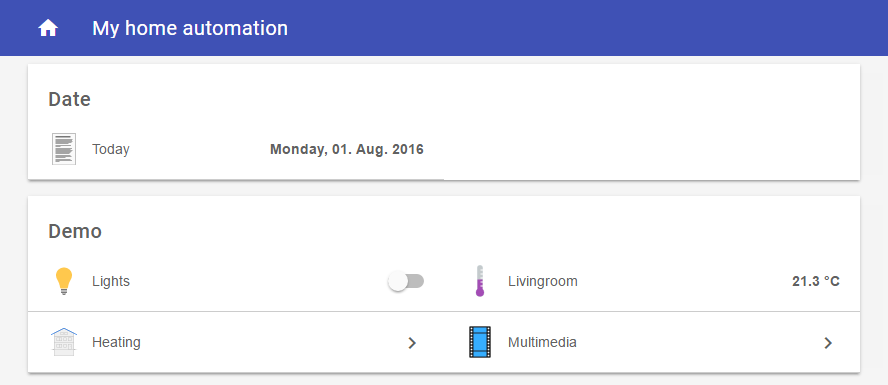
\includegraphics[width=12cm]{Immagini/SitemapViewExample}
    \caption{Esempio di View di una Sitemap}
    \label{fig:sitemap_view_example}
\end{figure}

\paragraph{Elements} le {\em sitemaps} sono composte da vari elementi. L'esempio contiene come elementi {\em Frame}, {\em Text} e {\em Switch}. Gli elementi presentano informazioni, consentono l'interazione e sono altamente configurabili in base allo stato del sistema. Una riga di definizione dell'elemento della {\em sitemap} produce un elemento dell'interfaccia utente corrispondente. Come mostrato nell'esempio, ogni elemento genera un testo descrittivo accanto a un'icona sul lato sinistro e uno stato e/o elementi di interazione sulla destra.

\paragraph{Parameters} è possibile configurare un determinato set di parametri per personalizzare la presentazione di un elemento. Nell'esempio mostrato {\em item} e {\em label} sono parametri. Quasi tutti i parametri sono opzionali, alcuni sono tuttavia necessari per ottenere un'interfaccia utente significativa. Per evitare righe di definizione degli elementi molto lunghe o non strutturate, i parametri possono essere suddivisi in più righe di codice.

\paragraph{Blocks} incapsulando gli elementi con parentesi graffe, è possibile annidare più elementi all'interno di altri. Il tipo di elemento {\em Frame} viene spesso utilizzato in combinazione con i blocchi di elementi. I frame vengono utilizzati per distinguere visivamente più elementi dello stesso argomento su una pagina dell'interfaccia. Quando si utilizzano blocchi di codice con altri tipi di elementi come {\em Text} o {\em Group}, questi elementi dell'interfaccia utente, oltre alla loro normale funzione, saranno collegamenti a una nuova vista, presentando gli elementi nidificati. Nell'esempio precedente, sono definiti più {\em Frame} e alcuni elementi non sono visibili nella vista principale ma sono accessibili dietro il loro elemento genitore. Questi sono indicati dall'icona di controllo ``\textgreater" a destra di un elemento.

\paragraph{Dependencies} una tipica {\em sitemap} contiene dozzine di singoli elementi. Lo stato del sistema e le possibili interazioni sono tuttavia spesso strettamente dipendenti. OpenHAB supporta queste dipendenze fornendo parametri per il comportamento dinamico.

L'elemento {\em sitemap} è obbligatorio nella definizione di una {\em sitemap}. Nell'esempio del Codice \ref{code:sitemap_code_example} alla riga 1 troviamo l'elemento {\em sitemap} con
\begin{itemize}
    \item {\em sitemapname} ovvero {\em demo}. Deve essere lo stesso nome del file, quindi il file contenete tale codice deve chiamarsi {\em demo.sitemap}.
    \item {\em label} ovvero {\em My home automation}. Esso è il testo della {\em sitemap} mostrato a video.
\end{itemize}

Gli elementi che possono essere utilizzati in una {\em sitemap} possono essere quelli della Tabella \ref{tab:sitemap_element_types}.

\begin{table}[]
    \centering
    \begin{tabular}{l|p{10cm}}
        \textbf{Element} & \textbf{Descrizione} \\
        \hline
        Chart & Aggiunge un oggetto grafico rappresentante una serie temporale per i dati persistiti\\
        Colorpicker & Permette l'utente di scegliere un colore da una color wheel\\
        Default & Esegue il rendering di un elemento nella rappresentazione dell'interfaccia utente predefinita specificata dal tipo di elemento specificato\\
        Frame & Stabilisce un'area contenente vari altri elementi della sitemap\\
        Group & Concentra tutti gli elementi di un dato gruppo in un blocco annidato\\
        Image & Rende un'immagine data da un URL\\
        Mapview & Visualizza una mappa OSM basata su un determinato elemento posizione\\
        Selection & Fornisce un menu a discesa o un popup modale che presenta i valori tra cui scegliere per un elemento\\
        Setpoint & Rende un valore compreso tra i pulsanti di aumento e diminuzione\\
        Slider & Presenta un valore in un cursore simile a una barra di avanzamento\\
        Switch & Rende un oggetto come interruttore ON/OFF o multi-pulsante\\
        Text & Rende un oggetto come testo\\
        Video & Visualizza un flusso video, dato un URL\\
        Webview & Visualizza il contenuto di una pagina web
    \end{tabular}
    \caption{Tipi di Elementi di una Sitemap}
    \label{tab:sitemap_element_types}
\end{table}

\section{Modello Semantico}
Uno degli scopi di openHAB è quello di astrarre gli smart device vedendoli nel modo più generico possibile così da mantenere una logica semplice e facilmante gestibile con l'annessione di qualsiasi altro dispositivo. Proprio per questo vengono usati gli {\em items} che nascondono l'oggetto fisico. Essi sono le entità principali con le quali lavorano le API Rest di openHAB. I vari {\em items} vengono raccolti in un modello semantico che permette di organizzarli in maniera semplice ed intuitiva in modo tale da semplificare l'uso da parte dell'utente.

\begin{figure}
    \centering
    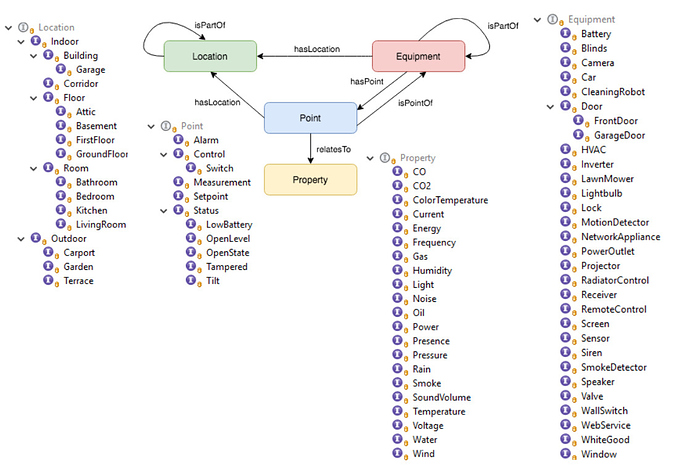
\includegraphics[width=12cm]{Immagini/ontology_relationships}
    \caption{Relazioni Ontologiche}
    \label{fig:ontology_relationships}
\end{figure}

Come rappresentato all'esempio della Figura \ref{fig:ontology_relationships} vi sono 4 concetti fondamentali nel modello semantico
\begin{itemize}
    \item \textbf{Location} è un {\em group item} che può contenere altre location, equipments e points e rappresenta una posizione fisica (edificio, stanza, ...). Una Location può essere membro di un solo Location Group
    \item \textbf{Equipment} è normalmente un {\em group item} che può contenere un equipment secondario e points. Un Equipment può essere membro diretto di una sola Location o un solo Equipment
    \item \textbf{Point} non è un gruppo, ma rappresenta qualsiasi altro tipo di elemento ed è solitamente collegato a un channel. Un Point può essere membro diretto di una sola Location o un solo Equipment
    \item \textbf{Property} è un tag aggiuntivo su un point item che indica che tipo di punto è (esempio: un termometro potrebbe essere un point di tipo misurazione con una property di tipo temperatura)
\end{itemize}

A Figura \ref{fig:example_model} vi è un esempio avanzato di modello.
\begin{figure}
    \centering
    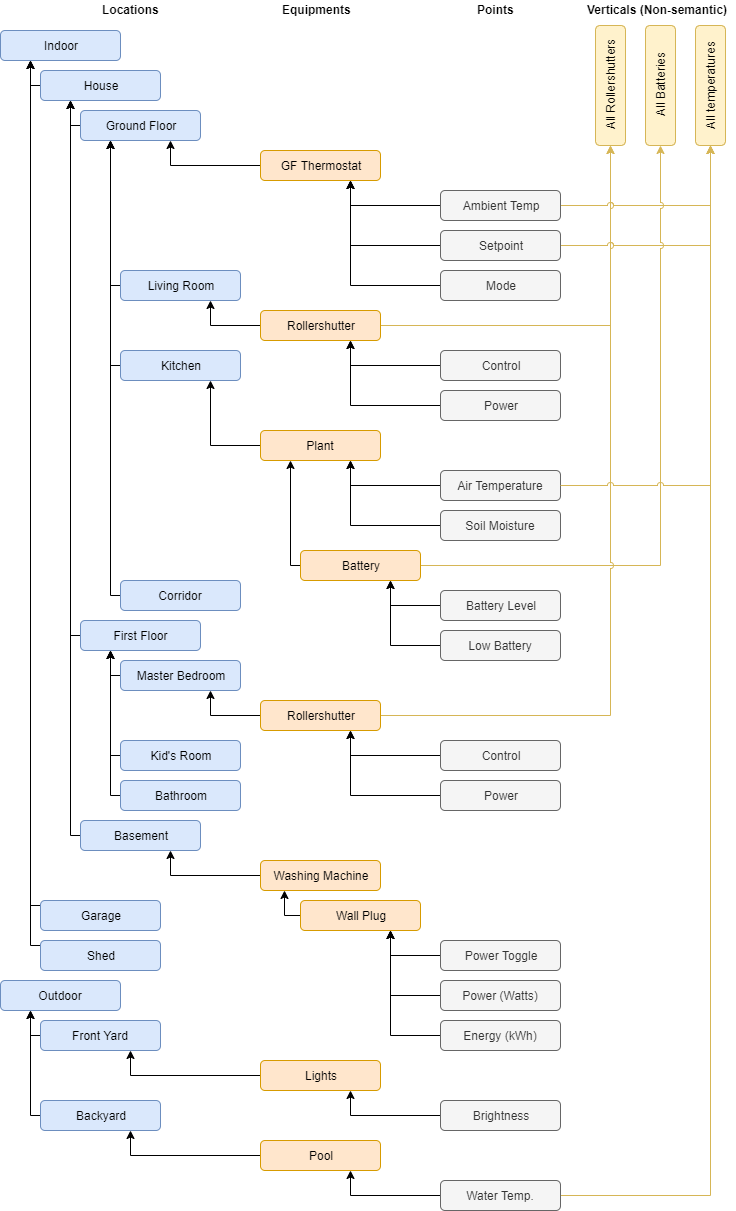
\includegraphics[width=12cm]{Immagini/example_model}
    \caption{Esempio di Modello}
    \label{fig:example_model}
\end{figure}

\section{Persistence}
OpenHAB permette di tenere traccia degli stati storici degli {\em items} attraverso l'uso della persistenza. Con essa quindi si può 
\begin{itemize}
    \item Tracciare un grafico della lettura di un sensore di temperatura nel tempo
    \item Ripristinare un elemento allo stato che aveva prima della chiusura o del riavvio di openHAB
    \item Usare lo stato di un oggetto nel passato, o qualche aggregato dello stato di un oggetto nel passato (esempio: Media da un'ora fa) nelle regole di automazione 
\end{itemize}

Per persistere i dati vengono forniti più database sia interni che esterni. Quelli esterni richiedono l'installazione e la configurazione su server separato.

Quando {\em persistence} salva gli stati degli {\em items}?
\begin{itemize}
    \item quando un {\em item} cambia
    \item quando un {\em item} viene aggiornato
    \item quando un {\em item} riceve un comando
    \item ogni minuto se ha ricevuto un evento
\end{itemize}

Una strategia di persistenza è {\em restoreOnStartup} che permette di aggiornare gli {\em items} con gli stati salvati più recentemente. Può essere possibile creare nella cartella  \\\textbf{\$OH\_CONF/persistence} un file con estensione {\em .persist} per definire la strategia di persistenza. 

Il database predefinito per la persistenza è \texttt{rrdj4} e viene fornito con strategie {\em everyChange}, {\em everyMinute} e {\em restoreOnStartup}. La comodità di questo database è che rimane sempre di una dimensione preimpostata e non c'è bisogno di pulirlo. Per eseguire tale logica rimpiazza i vecchi records con quelli nuovi. Questo approccio non funziona con tutti i tipi di {\em items}.

\section{openHAB REST API}
Tramite le REST API di openHAB è possibile accedere alla piattaforma da altre applicazioni e manipolare i dati visti nella struttura. Ciò include l'accesso ad {\em Item}, {\em Things} e {\em Bindings} e la modificazione dei vari stati. Le interazioni con l'API REST si basano su protocollo {\em http}. \'E possibile accedere tramite {\em internet} all'API REST ma a discapito della sicurezza, poiché in tale modo si espone openHAB a chiunque è in rete. Gli utenti infatti sono incoraggati a garantire connessioni sicure e protette. {\em OpenHAB API REST} può non essere installata automaticamente ma una volta fatto è accessibile tramite la dashboard.

Esempi di applicazioni di REST API in openHAB sono
\begin{itemize}
    \item Recupera i dati openHAB da applicazioni esterne
    \item Inietta dati e attiva eventi in openHAB da applicazioni esterne (esempio: alcuni rilevatori di movimento o telecamere di sorveglianza)
    \item Ispeziona bindings, things o items di openHAB, scopri gli states, i parametri o i problemi correnti
    \item Interagire con openHAB da altri programmi; molti linguaggi di programmazione e strumenti di automazione possono facilmente utilizzare l'API REST
    \item Utilizzo di software di terze parti sui telefoni cellulari, come tasker per aprire la porta del garage
\end{itemize}

Esempi di applicazione pratica tramite il tool {\em curl} che permette di fare chiamate REST al servizio server
\begin{itemize}
    \item Commutazione My\_ItemOFF mediante l'emissione di un HTTP POST richiesta
    \begin{lstlisting}
    curl -X POST --header "Content-Type: text/plain" --header "Accept: application/json" -d "OFF" "http://{openHAB_IP}:8080/rest/items/My_Item"
    \end{lstlisting}
    \item Impostare una voce di contatto My\_Item su CHIUSO emettendo una richiesta http PUT a My\_Item/state
    \begin{lstlisting}
    curl -X PUT --header "Content-Type: text/plain" --header "Accept: application/json" -d "CLOSED" "http://{openHAB_IP}:8080/rest/items/My_Item/state"
    \end{lstlisting}
    \item Recupero di un elenco di tutti gli items e groups mediante l'emissione di una richiesta GET
    \begin{lstlisting}
    curl -X GET --header "Accept: application/json" "http://{openHAB_IP}:8080/rest/items?recursive=false"
    \end{lstlisting}
    \item Recupero di un elenco di tutte le sitemap mediante l'emissione di una richiesta GET
    \begin{lstlisting}
    curl -X GET --header "Accept: application/json" "http://{openHAB_IP}:8080/rest/sitemaps"
    \end{lstlisting}
    \item Iscrizione agli eventi
    \begin{lstlisting}
    curl "http://{openHAB_IP}:8080/rest/events?topics=smarthome/things/{thingUID}/statuschanged"
    curl "http://{openHAB_IP}:8080/rest/events?topics=smarthome/channels/{channelUID}/triggered"
    \end{lstlisting}
\end{itemize}

OpenHAB supporta anche la protezione tramite password per contenuti sensibili come parti del modello semantico. I meccanismi forniti per tale scopo sono l'{\em basic authentication} e l'{\em OAuth authorization}. La maggior parte dei linguaggi di programmazione già supporta queste tecnologie. Per aggiungere utente e password nelle chiamate {\em curl} basta aggiungere \texttt{-u \{USER\_NAME\}} e poi inserire la password richiesta. Per fare tutto con un singolo comando basta aggiungere \texttt{-u \{USER\_NAME:PASSWORD\}}. Con l'API token basta aggiungere il comando \texttt{-u \{API\_TOKEN\}}.

\'E possibile creare un API Token dal proprio profilo accedendo con username da amministratore e password, andando sul profilo e premendo su \texttt{Create new API token}. Illustrazione a Figura \ref{fig:apitoken_login}.

\begin{figure}
    \centering
    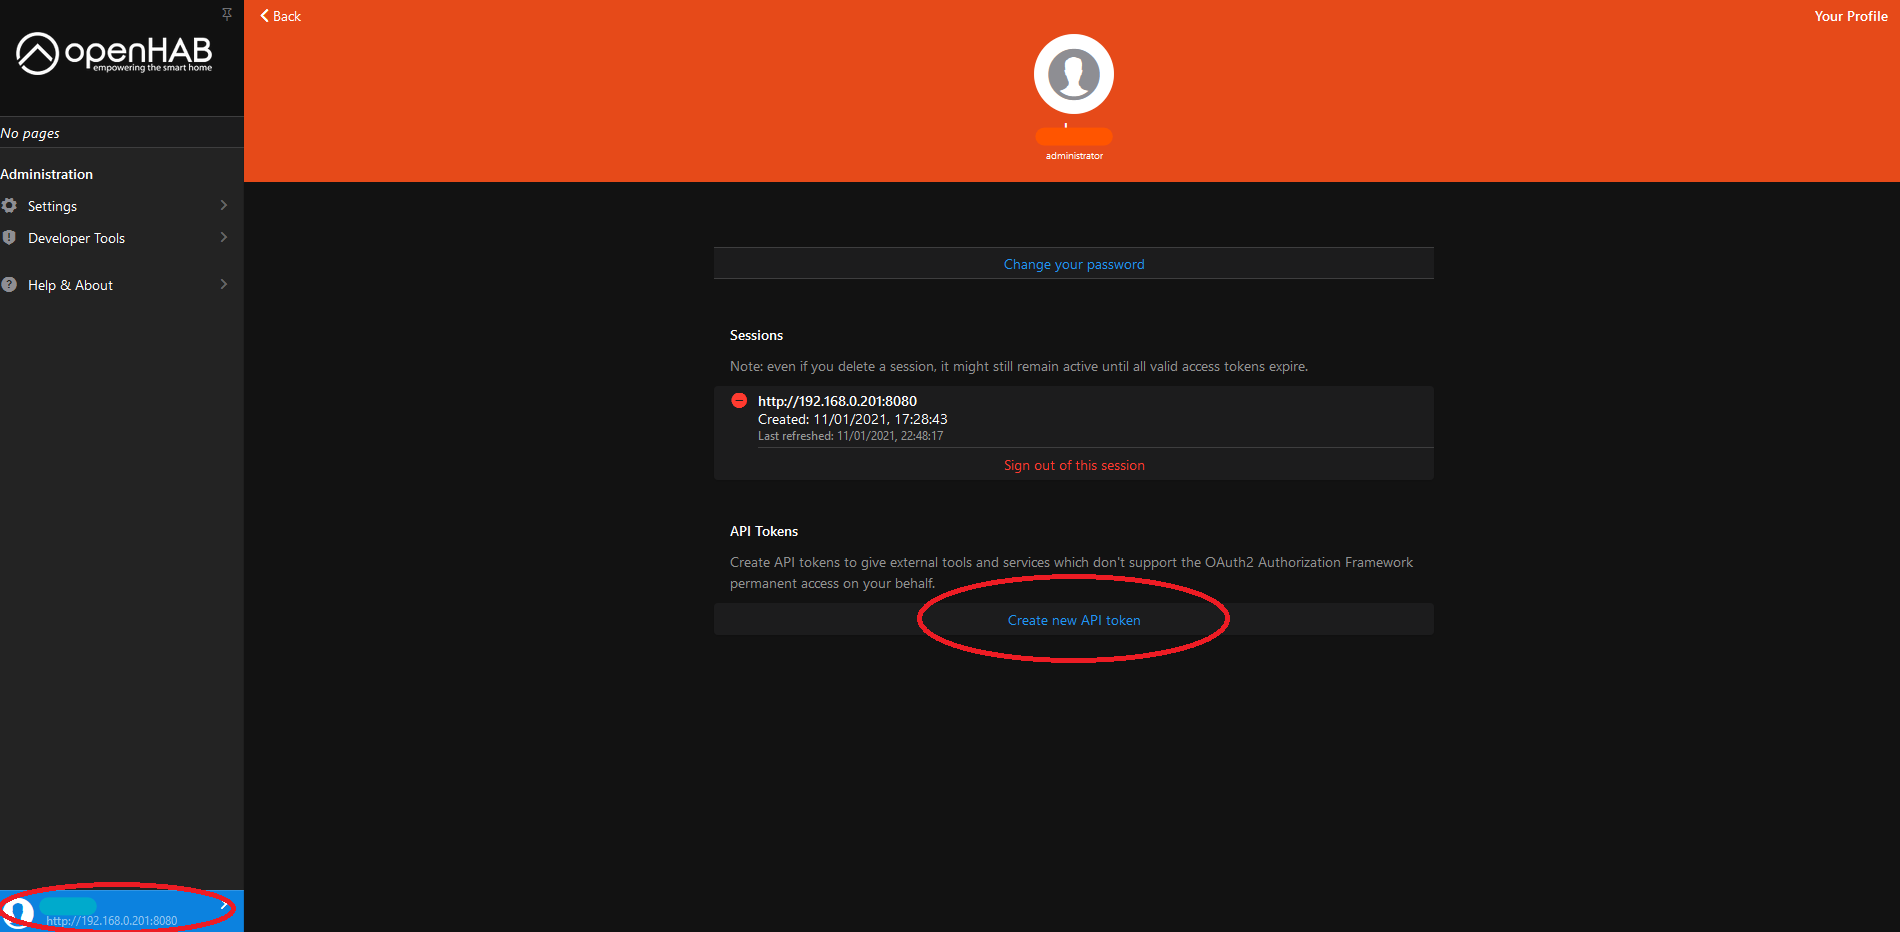
\includegraphics[width=14cm]{Immagini/apitoken_login}
    \caption{API Token Login}
    \label{fig:apitoken_login}
\end{figure}